\section{Background}
\label{sec:background}

\begin{figure}[t]
\centering
\begin{tikzpicture}
\matrix[square matrix]
{
W & W & W      & \tiny W,E & E & E & E  \\ 
  %W & W & W      & \tiny W,E & E & |[fill=lightgray]| E & E  \\ 
  W & W & W      & \tiny W,E & E & E & E  \\ 
  W & W & |[fill=black]|  & |[fill=black]|  & |[fill=black]|   & E & E  \\ 
  W & W & W      & |[fill=yellow]| $s$  & E & E & E  \\ 
  \tiny W,SW & \tiny W,SW & SW& S  & SE & \tiny E,SE & \tiny E,SE \\
};
\end{tikzpicture}
\caption{
\label{fig:g}
This first-move table records all optimal moves (cf. just one) 
from the source node $s$ to each traversable
(white) cell $t$.  
}
%\pjs{Tricky. Have to change the CPD to return a MOVE in order for reverse CPDS to work!}
\end{figure}  


We present background information on gridmaps, compressed path databases and wildcards,
that are necessary to understand the new contributions of this paper.

\paragraph{Gridmaps.} 
A gridmap is a two-dimensional data structure that represents the operating
environment for a mobile agent, such as a robot or a game character.
Gridmaps rasterise the environment into square cells, with each cell being 
either traversable or blocked. 
Each cell has up to 8 neighbours: one in each of the four cardinal 
(equiv. straight) directions and one in each of the four ordinal
(equiv. diagonal) directions.

When moving, each agent occupies exactly one traversable cell at a time and 
each is allowed to step to any other adjacent traversable cell.
Straight moves have a cost of 1, while diagonal moves cost $\sqrt{2}$. 
We further enforce the {\em no-corner-cutting rule}, which says that 
diagonal moves are disallowed if the origin and destination cell share a 
common neighbour which is not traversable.

Given a grid cell $n$, we write $n.x$ and $n.y$ for the $x$ and $y$ 
coordinates of that cell.
Further, let $MV = \{$ N, NE, E, SE, S, SW, W, NW $\}$ be the set of 8 
principal compass directions in which the agent can move.
Given a move $m \in MV$ and cell $n$ we define $m(n)$ as the node 
$n'$ where $n'.x = n.x + horiz(m)$ and $n'.y = n.y + vert(m)$
where
$$
horiz(m) = \left\{ \begin{array}{ll}
                    -1 & m \in \{\mbox{SW, W, NW}\} \\
                    0  & m \in \{\mbox{N, S}\} \\
                    +1 & m \in \{\mbox{NE, E, SE}\}
                    \end{array}\right.
$$
$$
vert(m) = \left\{ \begin{array}{ll}
                    -1 & m \in \{\mbox{NW, N, NE}\} \\
                    0  & m \in \{\mbox{E, W}\} \\
                    +1 & m \in \{\mbox{SE, S, SW}\}
                    \end{array}\right.
$$

Notice that each gridmap induces an undirected graph where traversable 
cells are nodes, and the moves applicable in each traversable cell are edges. 
Consider then a weighted
graph $G = (V,E)$ with vertices $V$ and edges $E \subseteq V \times V$,
and a function $w$ such that $w(s,t)$ is the cost of edge
$(s,t) \in E$.
\ignore{
A \emph{path} from $s$ to $t$ in $G$ is a sequence of edges
[$(n_0,n_1)$, $(n_1,n_2)$, \ldots, $(n_{k-1},n_k)$], where $k \in \mathbb{N}^+$, $n_0 = s$, and $n_k = t$.
The length of the path is $\sum_{i=0}^{k-1} w(n_i,n_{i+1})$.
}

A \emph{path} $p$ from $s$ to $t$ in $G$ is a sequence of nodes
[$n_0,n_1,n_2, \ldots, n_{k-1},n_k$], where $k \in \mathbb{N}^+$, $n_0 = s$, $n_k = t$, and $(n_i,n_{i+1}) \in E, 1 \leq i < k$.
The \emph{length} of the path is $len(p) = \sum_{i=0}^{k-1} w(n_i,n_{i+1})$.
The \emph{reverse}  $rev(p)$ of the path $p$ is the reverse sequence of its nodes.
Let $sp(s,t)$ return a shortest length path in $G$ from $s$ to $t$.
We use symbol $\pp$ to denote sequence (and thus also path) concatentation.

%\ignore{
\begin{algorithm}[t]
  \caption{Function $cpd$($s, t$) extracts at runtime an
  optimal path from the node $s$ to the node $t$.}
  \label{alg:retrieve}
$p \gets [s]$ \\
\While{$s \neq t$}
      {

      $m \gets \emptyset$\\
      \If{ $t$ is in the proximity square of $s$ }
      {
         $m \gets F_x(s, t)$
      }
      \Else
      {
      $m \gets$ \textsf{FirstMove}($s,t$) \\
      \If{$m = \heur$}
      {$m \gets F_x(s,t)$}
      }

      $p \gets p\, \pp\, [m(s)]$ \\ 
      $s \gets m(s)$
      }
\Return $p$
\end{algorithm}
%}

\paragraph{Compressed Path Databases (CPDs).} A CPD is a
data structure for encoding the first edge or move $m$ on
an optimal path, from any node $s$ to any node $t$ --- i.e., $(s,m(s))$.
%In this paper, we use the terms ``edge'' and ``move'' interchangeably.
%Likewise for ``cell'' and ``node'' and ``gridmap'' and ``graph''.
%In the rest of this section we review key aspects of CPDs that are 
%necessary to understand the new contributions presented later in this paper.

%path planning on gridmaps.  In this section we introduce the
%core components introduced in previous work~\cite{botea-aiide11,strasser-et-al-2014,DBLP:conf/aips/SalvettiBSG1, ????}


%The essence of a compressed path database is a data structure
%that allows us to
%quickly extract for any pairs of points $s$ and $t$
%in the graph a
%first edge to take from $s$ in order to reach $t$ optimally.

CPDs are constructed {\em offline} in a preprocessing phase 
that requires repeated iterations of Dijkstra search: 
one per graph node.
With only slight modifications, this algorithm can be used 
to produce an array $T(s)$ which records {\em all} optimal
first moves, from the source node $s$ to any reachable
target $t$. 
This array is sometimes called a {\em first-move table}.
Once computed, $T(s)$ is compressed and stored, which
concludes the iteration at hand.
Our compression scheme is based on run-length
encoding (RLE) of each first move table.
The algorithm is simple~\cite{strasser-et-al-2014}, but we 
omit a complete description for brevity.
%Figure~\ref{fig:g} shows an example.
Notice that, being independent, each Dijkstra iteration can be 
executed in parallel, with a speed-up linear in the number of
available processors.

\begin{example}\label{ex::first-move-table}
Consider the gridmap shown in Figure~\ref{fig:g}. RLE compresses a
string of symbols by representing more compactly substrings, called runs,
consisting of repetitions of the same symbol. E.g., the substring W; W; W;
(W,E); E; E; E (the first row in the figure) can have two runs, namely 
WWWW, and EEE. 
We replace each such run by a pair of values: one value indicates 
the starting index (where the run begins) and the other value stores the 
associated symbol. With RLE the example substring can be represented more 
efficiently as 1W; 5E.  
%
Overall, the entire string is compressed into 11 runs: 1W 5E 8W 12E 15W 20E 22W 26E
29SW 32S 33SE. Note that obstacle nodes and the source are assigned
{wildcard symbols}~``$*$''; i.e., ``don't care'' symbols,
because we never need to look up a move from \emph{s} to any of these.
%
Storing all optimal moves improves run-length 
compression, since any of the available symbols can be used
to extend runs.
E.g., observe how we are free
to choose any symbol from a non-singleton list such as (W,E). 
%%This is even
%%more clear for the last three elements at the end of the string: SE; (E,SE);
%%(E,SE). These are compressed into a run of three copies of the SE
%%symbol.
%
The size of the CPD can be further reduced by organising the columns
of each first move table according to a global ordering. We use the
DFS ordering scheme suggested in~\cite{strasser-et-al-2014}.
\end{example}

%\begin{comment}
%We restrict ourselves in the presentation to octile
%grid graphs where each node $n$
%has an $x$ coordinate $n.x$ and a $y$ coordinate $n.y$
%and has the 8 possible edges named
%$N$, $S$, $E$, $W$, $NE$, $NW$, $SE$, and $SW$.
%Note in this case diagonal edges have length $\sqrt{2}$ and
%cardinal edges have length 1.
%We will use these to name edges, e.g. the E edge from
%the node at (5,2) goes to the node at (5,3)
%The ideas are generalisable to any graphs where
%although some of the heuristics we use are specialised for grid graphs.
%\end{comment}
%
%\ignore{
%\begin{example}
%  \label{ex::first-move-table}
%  Consider the gridmap shown in Figure~\ref{fig:g}.
%  We illustrate an iteration of the preprocessing
%%  Consider the gridmap shown in Figure~\ref{fig:g},
%%  where black cells are obstacles (blocked cells)
%%  and all other cells are traversable.
%%  We illustrate an iteration of the preprocessing
%  that builds the CPD.
%  In our example, Dijkstra is run from the source node
%  \emph{s}. For each traversable cell we now specify all the 
%  optimal first moves, from \emph{s} to the node at hand.
%For example, two optimal first moves exist from \emph{s} towards the bottom-left corner: W and SW.
%%  For example, the (only) first optimal move from $s$ towards
%%  the top-left corner is W.
%%  Two first optimal moves exist from $s$ towards the bottom-left corner: W and SW.
%% After all these optimal moves are found with the Dijkstra search from $s$,
%%the set of optimal moves is compressed.
%  %
%Compressing the set of first-moves requires a fixed ordering of the graph nodes.  
%%Compression requires a fixed ordering of the graph nodes.
%  In our example we assume that the nodes are ordered
%  left to right and top to bottom.
%%  According to that ordering, the string of optimal moves is:
%%  W; W; W; (W,E); E; E; E; W; W; W; (W,E); E; E; E; W; W; $*$; $*$; $*$; E; E; W; W; W; $*$; E; E; E; (W,SW); (W,SW); SW; S; SE; (E,SE); (E,SE).
%
%%
%}


%\ignore
%{
%Following the approach of
%\citeauthor{strasser-et-al-2014}~\shortcite{strasser-et-al-2014}, the string
%of symbols is encoded with run-length encoding (RLE). RLE compresses a
%string of symbols by representing more compactly substrings, called runs,
%consisting of repetitions of the same symbol. E.g., the substring W; W; W;
%(W,E); E; E; E (the first row in the figure) can have two runs, namely 
%WWWW, and EEE. 
%We replace each such run by a pair of values: one value indicates 
%the starting index (where the run begins) and the other value stores the 
%associated symbol. With RLE the example substring can be represented more 
%efficiently as 1W; 5E.  Observe how we are free
%to choose any symbol from a non-singleton list such as (W,E). 
%%This is even
%%more clear for the last three elements at the end of the string: SE; (E,SE);
%%(E,SE). These are compressed into a run of three copies of the SE
%%symbol.
%Overall, the entire string is compressed into 11 runs: 1W 5E 8W 12E 15W 20E 22W 26E
%29SW 32S 33SE. Note that obstacle nodes and the source are assigned
%{wildcard symbols}~``$*$''; i.e., ``don't care'' symbols,
%because we never need to look up a move from \emph{s} to any of these.
%This concludes one iteration of CPD preprocessing.
%
%Once preprocessing is complete the resulting CPD can be used to 
%look up optimal moves by performing a binary search
%on the compressed string of any given source node, as shown in Algoithm~\ref{alg:dec}. 
%For example, to
%look up the optimal move from \emph{s} to (6,2), the greyed location which is at index 13, 
%we start with end pointers $(l,u) = (1,11)$ and look up middle point $m = 6$, 
%which is the entry 20E.
%As $13 < 20$, the binary search continues to the left, setting $u = 5$.
%Next we look up $m = 3$ (the 8W entry in the compressed string) and
%since $13 \geq 8$, we continue to the right, setting $l = 3$. Next we
%look up $m = 4$ (entry 12E) and set $l = 4$. Next we look up $m =
%5$ (the 15W entry) and set $u = 4$. The search ends because $u \leq l$.
%The search returns move E of the fourth entry 12E.
%\end{example}
%}



With a CPD in hand, we may begin the {\em online} phase of the algorithm.
Here the objective is to compute optimal paths and prefixes for any given
start-target pair (equiv. {\em instance}).
We denote as \textsf{FirstMove}($s$,$t$) the function which returns an 
optimal first move from $s$ to $t$.
The implementation of this function requires a simple binary 
search through a compressed string of symbols~\cite{strasser-et-al-2014}.
The function can be used to extract entire optimal paths or optimal
prefixes of any given size.
In this work we compute optimal paths using Algorithm~\ref{alg:retrieve}. 
The method relies on two recent 
optimisations~\cite{icaps19b} which are known to improve efficiency: 
Heuristic Moves and Proximity Wildcards. We describe these next.

%
%\begin{comment}
%\begin{algorithm}
%  \caption{\small Building a CPD}
%  \label{alg:cpd}
%  \For{each $n \in V$}
%      { $T \gets \textsf{Dijkstra}(n)$ \\
%        $L(n) \gets \textsf{Compress}(T)$ }
%\end{algorithm}
%\end{comment}
%
%\pjs{We need to talk about column ordering somewhere?}
%
%\begin{comment}
%We build a CPD using Algorithm~\ref{alg:cpd}.
%After applying \textsf{Dijkstra} we have an array
%$T$ for node $n$ which for each target node $t$
%returns a list of all possible first moves
%which lead to a shortest path to node $t$.
%Note that the fact that $T(t)$ may not be a singleton is important
%for obtaining maximum compression.
%We assume that $T(t)$ returns all possible moves (represented by $*$)
%for nodes $t$ which are not reachable from $n$ or are equal to $n$.
%\pjs{Actually what dose happen for non-connected graphs}
%
%We will compress the \emph{array} of first possible moves using
%run length encoding.
%In order to use run length encoding we must totally order the nodes $V$
%in the graph.  We assume a bijective
%mapping $col: V \rightarrow 1..|V|$ which maps
%each node to a unique column number in $1 .. |V|$.
%The run length encoding encodes the nodes in the order given by this mapping,
%and the column number is used to extract information about a node.
%There are a number of approaches to choosing a column order
%in order to shrink the resulting run length encoding which are
%discussed by ?????~\cite{}
%In the experiments we will use two: \textsf{dfs} and \textsf{cut}
%while in the presentation we will simply use the natural node order.
%
%The compression algorithm (Algorithm~\ref{alg:rle})
%uses run length encoding
%to encode one possible correct move for each integer from
%$1 .. | V|$ where the $c^{th}$ entry represents the
%node $t$ where $col(t) = c$ .
%It computes the intersection $S$ of all moves in a sequence starting from
%column $f$ until this becomes empty $S' = \emptyset$.
%We then encode the
%previous run as $f m$ where $m \in S$ and $f$ is the first column in the run,
%and start collecting the new set of possible symbols. 
%
%\pjs{1-based indexing of nodes and arrays or 0-based indexing!}
%
%\begin{algorithm}
%  \caption{\small Optimal Run Length Encoding of CPD}
%  \label{alg:rle}
%  \textsf{Compress}($T$) \\
%  $i \gets 1$ ;  $c \gets 1$; $f \gets 1$ \\
%  $S \gets T(col^{-1}(c))$ \\
%  \While{$c \leq |V|$}
%    { $c \gets c + 1$ \\
%      $S' \gets S \cap T(col^{-1}(c))$ \\
%    \If{$S' = \emptyset$}
%       { \textrm{choose} $e \in S$ \\
%         $D[i] \gets (f, e)$ \\
%         $i \gets i + 1$ \\
%         $S' \gets T(col^{-1}(c))$ \\
%         $f \gets c$ 
%       }
%      $S \gets S'$
%    } 
%    \textrm{choose} $e \in S$ \\
%    $D[i] \gets (f, e)$ \\
%    \Return $D$
%\end{algorithm}
%
%\ab{Algorithm \ref{alg:rle} is not necessary.
%Communicating the idea of this algorithm with an example
%would be better.}
%\end{comment}
%%         
%The decoding of the CPD (Algorithm~\ref{alg:dec})
%uses binary search across the run length array
%to find the move attached to a certain location $t$.
%%It makes use of the accumulated counts to find the decoding
%%for any location.
%%\pjs{Actually dont use the counts!}
%
%\ignore
%{
%\begin{algorithm}
%  \caption{\small Decoding the Run Length Coding \textsf{CPD}($s,t$)
%}
%  \label{alg:dec}
%  $D \gets L(s)$ \\
%  $c \gets col(t)$ \\
%  $l \gets 1$ \\
%  $u \gets |D|$  \\
%  \While{$l < u$}
%        { $m \gets \lceil \frac{l+u}{2} \rceil$ \\
%          $(f, e) \gets D[m]$ \\
%        \eIf{$c \geq f$}
%           {$l \gets m$}
%           {$u \gets m-1$}
%           
%   }        
%   $(f, e) \gets D[l]$ \\        
%   \Return $e$        
%\end{algorithm}
%}
%%
%To extract a complete shortest path we repeatedly apply the CPD function until the target
%is reached.  The complete procedure is shown in Algorithm \ref{alg:retrieve}.
%
%%\begin{minipage}{\columnwidth}
%
%\ignore{
%\begin{algorithm}
%  \caption{Bidirectional path extraction at runtime for an ($s,t)$ pair}
%  \label{alg:wild}
%$\mbox{prefix} \gets []$ \\
%$\mbox{suffix} \gets []$ \\
%\While{$s \neq t$}
%      {\eIf{$(s,t) \in R$}
%           {$(s,n) \gets$ \textsf{CPD}($s,t$) \\
%             $\mbox{prefix} \gets \mbox{prefix} + [(s,n)]$ \\
%             $s \gets n$ }
%           {$(t,n) \gets$ \textsf{CPD}($t$,$s$) \\
%             $\mbox{suffix} \gets [(n,t)] + \mbox{suffix}$ \\
%        $t \gets n$}
%      }
%\Return $\mbox{prefix} + \mbox{suffix}$
%\end{algorithm}
%}
%\end{minipage}

%In practice, the size of the CPD can be reduced by choosing a
%\emph{column ordering}, that is the order in which nodes appear in
%the run length encoding. 
%
%For simplicity, in the running examples we will use a default
%order (left to right, top to bottom).
%However, in the experiments we use state-of-the-art 
%heuristic orderings introduced in previous work~\cite{strasser-et-al-2014}.
%These have been shown to outperform naive orderings in terms of memory
%by up to a factor of 10~\cite{DBLP:journals/jair/StrasserBH15}.


%,  an ordering based on depth-first
%traversal pre-order
%is typically 5 times better
%than the default order \cite{strasser-et-al-2014} \ale{CHECK!}.

\ignore{
\paragraph{Bidirectional Wildcards.}
%Salvetti~\emph{et al}~\cite{wildcards} 
\citeauthor{DBLP:conf/aips/SalvettiBSG17}~\shortcite{DBLP:conf/aips/SalvettiBSG17}
show how we can improve
the compression in a CPD for undirected graphs
by taking into account the duplicate information.
In order to find a shortest path from $s$ to $t$ we only need
to know either (a) the first move from $s$ towards $t$, or
(b) the first move from $t$ towards $s$.
We do not need both.

Assume a realised relation $R \subseteq V \times V$ which
defines which pairs of $(s,t)$ are realised correctly in the CPD.
For the completeness of path finding we simply require that
$\forall s \in V,
t \in V, s \neq t \rightarrow ((s,t) \in R \vee (t,s) \in R)$.

Given this information we can extract a shortest path from
$s$ to $t$ using a bidirectional search shown in Algorithm~\ref{alg:wild}.


In practice the realised relation $R$ is based on a
node ordering $\prec$,
so that $(s,t) \in R \Leftrightarrow s \prec t$.

The advantage of the realised relation is that if
$(s,t) \not \in R$ then we will never access the $t$ entry
in $L(n)$. Hence we can replace the entry in $T$ the
first moves array for $s$, $T(t)$ with wildcard entries ``$*$''.
This allows to create
more compressed run length encodings. % $L(s)$.
}

%\ab{In my opinion, the two columns with only wildcards don't help.  I suggest to remove them.}
%\pjs{I agree, although according to Daniel they do get column numbers!}

%\ignore{
%\begin{example}
%  Consider the graph shown in Figure~\ref{fig:w}. The $T$ arrays for each node are computed as
%$$
%  \begin{array}{l|ccccccccc}
%      & a  & b  & c  & d  &   &   & e  & f  & g \\ \hline
%    a & *  & E  & E  & S  & * & * & S  & S  & S \\
%    b & W  & *  & E  & SW & * & * & SW & SW & SW \\
%    c & W  & W  & *  & W  & * & * & W  & W  & W \\
%    d & N  & NE & NE & *  & * & * & S  & SE & SE \\
%    e & N  & N  & N  & N  & * & * & *  & E  & E \\
%    f & NW & NW & NW & NW & * & * & W  & *  & E \\
%    g & W  & W  & W  & W  & * & * & W  & W  & * \\
%  \end{array}
%$$
%  The run length encodings lead to
%  3E 8S, 2W 1E 6SW, 9W, 1N 5NE 1S 2SE, 7N 2E, 6NW 2W 1E, 9W
%  with a total of 16 entries.
%  If we assume the order $\prec$ defined by
%  $b \prec e \prec f \prec a \prec c \prec g \prec d$
%  then we replace all entries which do not respect the ordering by
%  $*$ obtaining the $T$ arrays
%$$
%  \begin{array}{l|ccccccccc}
%      & a  & b  & c  & d  &   &   & e  & f  & g \\ \hline
%    a & *  & *  & E  & S  & * & * & *  & *  & S \\
%    b & W  & *  & E  & SW & * & * & SW & SW & SW \\
%    c & W  & *  & *  & W  & * & * & *  & *  & W \\
%    d & *  & *  & *  & *  & * & * & *  & *  & * \\
%    e & N  & *  & N  & N  & * & * & *  & E  & E \\
%    f & NW & * & NW & NW  & * & * & *  & *  & E \\
%    g & *  & *  & *  & W  & * & * & *  & *  & * \\
%  \end{array}
%$$
%  The run length encoding is now 3E 6S, 2W 1E 6SW, 9W, 9*, 7N 2E, 8NW 1E, 9W
%  with a total of 12 entries.
%
%  To find a shortest path from $c$ to $f$, we find $c \not\prec f$
%  so lookup $CPD(f,c)$ to find a move NW $(f,d)$.  We find $c \prec d$
%  so lookup $CPD(c,d)$ to find a move W $(c,b)$. We find $b \prec d$
%  so lookup $CPD(b,d)$ to find a move SW $(b,d)$.
%  Since both ends are identical we finish.
%  The path discovered is $[(c,b),(b,d),(d,f)]$.
%  \begin{figure}
%    \centering
%    \begin{tikzpicture}
%   \matrix[square matrix]
%   {
%      $a$  & $b$  & $c$   \\
%      $d$ & |[fill=black]|  & |[fill=black]| \\
%      $e$ & $f$ & $g$  \\
%   };
%    \end{tikzpicture}
%    \caption{\small A small graph with named nodes.}
%    \label{fig:w}
%  \end{figure}  
%\end{example}
%
%  Note that the use of a realised relation is orthogonal to all
%  the other improvements we consider in this paper.
%
%
%  %\pjs{Just for my interest, I would try the order}
%  The order
%  $c \prec g \prec a \prec e \prec f \prec b \prec d$
%  leads to
%
%$$
%  \begin{array}{l|ccccccccc}
%      & a  & b  & c  & d  &   &   & e  & f  & g \\ \hline
%    a & *  & E  & *  & S  & * & * & S  & S  & * \\
%    b & *  & *  & *  & SW & * & * & *  & *  & * \\
%    c & W  & W  & *  & W  & * & * & W  & W  & W \\
%    d & *  & *  & *  & *  & * & * & *  & *  & * \\
%    e & *  & N  & *  & N  & * & * & *  & E  & * \\
%    f & *  & NW & *  & NW & * & * & *  & *  & * \\
%    g & W  & W  & *  & W  & * & * & W  & W  & * \\
%  \end{array}
%$$
%leading to encoding 3E 6S, 9SW, 9W, 9*, 7N 2E, 9NW, 9W with 9 entries!
%%}
%}

\paragraph{Heuristic Moves.}

%\begin{figure}[t]
%\centering
%\begin{tikzpicture}
%\matrix[square matrix]
%{
%  \bf W & \bf W & \bf W    & \bf E & \bf E & \bf E & \bf E  \\ 
%  \bf W & \bf W & \bf W    & \bf E & \bf E & \bf E & \bf E  \\ 
%  \bf W & \bf W & |[fill=black]|  & |[fill=black]|  & |[fill=black]|   & \bf E & \bf E  \\ 
%  \bf W & \bf W & \bf W      & |[fill=yellow]| $s$  & \bf E & \bf E & \bf E  \\ 
%  \bf SW & \bf SW & \bf SW & \bf S  & \bf SE & \bf SE & \bf SE \\
%};
%\end{tikzpicture}
%\caption{We show the \emph{h-moves} suggested by a default function $F_x(s,t)$; from the source
%node $s$ to all potential target nodes $t$. 
%All symbols are in bold, since each of them belongs to the corresponding set $T(t)$ for the marked symbol $s$.}
%\label{fig:h}
%\end{figure}

When pathfinding on a gridmap the first move from $s$ to 
$t$ is often the ``obvious move''; e.g., the move that heads 
directly towards the target or the one suggested by some ``default'' 
heuristic function $F_x(s, t)$.
%such as the Octile heuristic\footnote{Octile heuristic generalises
%the more well known Manhattan heuristic, from 4-connected grids to 
%8-connected grids.}.
In such cases we may add an extra ``redundant'' symbol $\heur$ to each 
applicable target node, after the completion of Dijkstra search but before compression
of the first-move table.
These additional symbols, sometimes called \emph{h-moves}, can be added to the
first move table in linear time and they significantly
improve the efficiency of CPDs; i.e. they help to reduce the 
total size of the database without impacting query performance.
%
E.g., by using the default heuristic function proposed by \citeauthor{icaps19b}~\shortcite{icaps19b}, the string of symbols shown in Figure \ref{fig:g} can be compressed into 1\heur. That is, the entire compressed string has only 1 run,
  which is substantially shorter than options discussed in Example~\ref{ex::first-move-table}.
  
Exploiting h-moves during the online stage requires only a small modification to
the standard path retrieval function: after extracting a $\heur$ symbol from
the CPD, we apply the move suggested by the default heuristic function.
%Figure~\ref{fig:h} shows an example.
Note that $\heur$ symbols are only applicable (i.e., only added to the first move table)
if the default heuristic returns just one possible move from $s$ to $t$.
Our implementation is based on \citeauthor{icaps19b}'s~\shortcite{icaps19b} algorithm and uses the
same heuristic.  
%We refer the interested reader to the original work for a full description.

\ignore{
Given nodes $s$ and $t$ we can define a \emph{default move} from $s$ to $t$, $d(s,t)$ as follows.
Let $A = [ NW, N, NE, W, \textrm{\it null}, E, SW, S, SE ]$ be the array of directions
indexed from 1 to 9.
Let $\sigma x = \sign(t.x - s.x)$, and $\sigma y = \sign(t.y - s.y)$, where $\sign(x)$ is $-1$ if $x <0$, $0$ if $x = 0$, and $+1$ if $x > 0$; then
$d(s,t) = A[\sigma x + 3\times \sigma y + 5]$.
Essentially, the default move is just the move that leads us
closest to the target, according to a heuristic distance function like, e.g., the Euclidean or the octile distance.
}

\ignore
{
When the default move $d$ from $s$ to
some node $t$ is one of the optimal first moves from $s$ to $t$,
i.e., if $d \in T(t)$ where $T$ is the first move array for $s$,
then we can encode this information in the CPD using the new symbol
$\heur$ which represents that we follow the heuristic of default moves.
Specifically, we add to $T(t)$ the new symbol $\heur$, in addition to the existing
contents of $T(t)$. This way, the compression step will have more options to 
choose what symbol to keep from $T(t)$ in the compressed string, with a potentially better compression in the end.
}

\ignore{
\begin{example}
  \label{ex::default-moves1}
  Consider the gridmap shown in Figure~\ref{fig:def}. For each node $t$, we show the
  default move bolded if it appears in $T(t)$ for $s$,
  that is the set of the optimal first moves sketched in Figure~\ref{fig:g.} As we can see, almost half of the graph can be encoded using the
  default moves. Once we add the heuristic move symbol $\heur$ to each
  entry $T(t)$ where the move is bolded, we can perform a better
  run length encoding.
  The encoding using the new heuristic move symbol is
  1W 5E 8W 12E 15W 20E 22\heur{}, which is smaller than without using \heur{
  (i.e., 7 runs in the new encoding, compared to 11 in Example~\ref{ex::first-move-table}).
  }
    \begin{figure}
    \centering
    \begin{tikzpicture}
   \matrix[square matrix]
   {
      NW & NW & NW    & N & NE & NE & NE  \\ 
      NW & NW & NW    & N & NE & NE & NE  \\ 
      NW & NW & |[fill=black]|  & |[fill=black]|  & |[fill=black]|   & NE & NE  \\ 
      \bf W & \bf W & \bf W  & |[fill=yellow]| $s$  & \bf E & \bf E & \bf E  \\ 
      \bf SW & \bf SW & \bf SW & \bf S  & \bf SE & \bf SE & \bf SE \\
   };
    \end{tikzpicture}
    \caption{The default first move $d(s,t)$ to each cell of the gridmap. Bold if it appears in $T(t)$ for the cell marked $s$.}
    \label{fig:def}
    \end{figure}
\end{example}

The heuristic move symbol is able to encode large parts of the graph which are
close to the source, and many other parts as well.

\subsection{Distance Functions}

The default move is quite basic, it takes no account of information
about the surroundings of $s$, and indeed in many cases the direction
returned may not even be possible.
We can improve the use of the heuristic move symbol \heur{} by
considering the relationship between $s$ and $t$ in more detail.
}

\ignore
{
How do we compute default moves?
Let $s$ be the source, $t$ be a target,
let $f_x(s,t)$ be a predefined heuristic distance function.
We assume $f_x(s,t)$ is simple to calculate.
%
For our examples we will use the octile distance function
%\begin{equation}
$$
\begin{array}{rcl}
f_o(s,t) & = & \sqrt{2} \times c + |s.x - t.x| - c + |s.y - t.y| - c \\
&& \mbox{~where~} c = \min (|s.x - t.x|, |s.y - t.y|)
\end{array}
$$
%\end{equation}

\noindent
or the Euclidean distance function

$$
%\begin{equation}
f_e(s,t)  =  \sqrt{(s.x - t.x)^2 + (s.y - t.y)^2}.
%\end{equation}
$$

%
We define the \emph{default move} chosen by the distance function
$F_x(s,t)$ from $s$ to $t$ as the move leaving $s$ to $n$ such that
the estimated path distance through $n$, 
$w(s,n) + f_x(n,t)$, is minimised, that is 
$$
F_x(s,t) = \argmin_{\hspace{-5mm}m \in MV, (s,m(s)) \in E} \{ w(s,m(s)) + f_x(m(s),t)\}. % ~|~ (s,n) \in E \}
$$
In order for $\heur$ to be used in the CPD, it
must be unambiguous, hence we assume a total
order on all moves leaving $s$,
and assume the $\argmin$ in $F$ returns the least
move in this order that leads to the minimal distance.
For gridmaps our default ordering is
NE, NW, SE,  SW, N, S, E, W.
Effectively this tries to take diagonal moves first when there is a tie.
}

\ignore{
The move chosen by the distance function is immediately better than the default move approach because
it can never choose invalid grid moves.
Just as before, if $F_x(s,t)$ returns a first move that corresponds with the
start of the shortest path from $s$ to $t$, then we can add the symbol
$\heur$ to the set $T(t)$ of possible first moves for $s$. 
}


\ignore
{
\begin{example}
  Consider the gridmap in Figure~\ref{fig:g}. 
  Figure~\ref{fig:h} shows the heuristic move to each node in the graph underlying the gridmap.
  Since for each target node $t$, $F_o(s,t) \in T(t)$ for $s$,
  we can add a heuristic move symbol $\heur$
  to each entry in $T(t)$.
  Now when we perform run length encoding we get the result
  1\heur. That is, the entire compressed string has only 1 run,
  which is substantially shorter than options discussed in Example~\ref{ex::first-move-table}.
\end{example}

The revised CPD lookup function is shown in Algorithm~\ref{alg:cpdh}.
It simply looks up the CPD as usual but, if it finds a symbol $\heur$, it
returns the default move $F_x(s,t)$, for whichever distance function 
we choose to use.

\begin{algorithm}
%\textsf{CPDH}($s$, $t$) \\
   {$m \gets$ \textsf{CPD}($s$,$t$) \\
     \eIf{$m = \heur$}
         {\Return $F(s,t)$}
         {\Return $m$}
         }
\caption{Get next move algorithm \textsf{CPDH}($s$, $t$) from $s$ to $t$ for CPDs with heuristic moves.}
\label{alg:cpdh}
\end{algorithm}
}

\paragraph{Proximity Wildcards.}
\citeauthor{icaps19b}~\shortcite{icaps19b} introduce a further use of heuristic moves by finding
the largest square around the start position $s$ where all moves can
be \heur{} and storing this information together with the compressed
list of symbols for each source node $s$. 
Before extracting a first move they check whether the target is within 
the square. If so, they simply apply the heuristic move.  
This speeds up the path extraction (since the lookup is constant time) and
helps to reduce the size of the database, since targets inside the
square can be treated as wildcards during compression (i.e., these targets
can be used to extend any existing run).
%We apply this optimisation to all CPDs computed in this paper.
%We make use of this for all forward CPDs in the paper.



\ignore{
\subsection{Improving the Tie-breaking}

The heuristic move must be unambiguous,
hence when there are moves that look equally good
we must choose one of them unambiguously.
This choice can be different for each source node $s$.
While the diagonal first ordering is a good default,
we can make use of the relative positions
of $s$ and $t$ to have better tie breaking.

\begin{example}
  Consider the gridmap in Figure~\ref{fig:i}. 
  We show the heuristic move $F_o(s,t)$
  to each cell of the gridmap in Figure~\ref{fig:i}(a),
  and the optimal first moves in Figure~\ref{fig:i}(b).
  Clearly all nodes can make use of a heuristic move, except those marked E
  on the second and third row.
  The resulting encoding is 1\heur{} 12E 13\heur{} 17E 19\heur{}.
  This pattern is common where some part of the graph
  is blocked.  We want to have a better tie breaker for such circumstances. 
  %
    \begin{figure}
      \centering
      \begin{tabular}{c@{~~~~~}c}
    \begin{tikzpicture}
   \matrix[square matrix]
   {
      |[fill=yellow]| $s$ & E & E  & E & E & E \\
      S & SE & SE    & |[fill=black]| & SE & SE \\
      S & SE & |[fill=black]|  & SE  & SE & SE  \\
      S & SE & SE      & SE  & SE & SE  \\
      S & SE & SE & SE  & SE & SE  \\
   };
    \end{tikzpicture}
    &
    \begin{tikzpicture}
   \matrix[square matrix]
   {
      |[fill=yellow]| $s$ & \bf E & \bf E & \bf E & \bf E & \bf E \\
      \bf S & \bf SE & \tiny E,\bf SE    & |[fill=black]| & E & E \\ 
      \bf S & \tiny S,\bf SE & |[fill=black]|  & \tiny S,\bf SE  & E & E  \\ 
      \bf S & \tiny S,\bf SE & \tiny S,\bf SE  & \tiny S,\bf SE  & \tiny S,\bf SE & \tiny S,\bf SE  \\ 
      \bf S & \tiny S,\bf SE & \tiny S,\bf SE & \tiny S,\bf SE  & \tiny S,\bf SE & \tiny S,\bf SE  \\
   };
    \end{tikzpicture} \\
    (a) & (b) 
      \end{tabular}
      \caption{(a) The heuristic first move $F_o(s,t)$ to each cell of the gridmap from the cell marked $s$
      and (b) the optimal first moves to each cell from $s$, with the heuristic moves in bold.}
    \label{fig:i}
    \end{figure}
\end{example}
  
%\pjs{Please add detailed descriptions of bytes-1, bytes-2?}

When we have blockages in the graph
it can often be the case that the heuristic best move
is not the diagonal move. We improve our heuristic tie breaking by breaking the graph
into 8 quadrants around $s$, corresponding to the 8 directions, and
break ties by choosing the closest direction to the
straight line direction from $s$ to $t$.
In order to avoid complex trigonometric operations
we use simple approximations:
if $|s.x - t.x| \geq 2|s.y - t.y|$ then the straight line from $s$ to $t$
is close to the horizontal line,
so we favour E or W, similarly if  $|s.y - t.y| \geq 2|s.x - t.x|$
then the straight line from $s$ to $t$
is close to vertical so we favour N or S.
In other cases we favour the closest diagonal direction. %\ale{It could be interesting to try with other rates different from 2.}
%\pjs{I know we tie break the other way, but it stuffs the example so leave it as is!}
%
We denote the heuristic move with directional tie breaking by $F^d_x(s,t)$
where $x$ denotes the distance function.

\begin{example}
  Consider the gridmap in Figure~\ref{fig:i} once more.
  Using direction-based tie breaking the heuristic moves are given in Figure~\ref{fig:j}.
  Note that now each heuristic move appears in the optimal first moves (Figure~\ref{fig:i}(b)),
  and hence we can encode all the first moves as 1\heur, that is much shorter than without using directional-based tie breaking.
  %
    \begin{figure}
      \centering
    \begin{tikzpicture}
   \matrix[square matrix]
   {
      |[fill=yellow]| $s$ & E & E  & E & E & E \\
      S & SE & E    & |[fill=black]| & E & E \\
      S & S & |[fill=black]|  & SE  & E & E  \\
      S & S & SE      & SE  & SE & SE  \\
      S & S & S & SE  & SE & SE  \\
   };
    \end{tikzpicture}
    \caption{The heuristic first move $F^d_o(s,t)$ to each cell of the gridmap from the cell marked $s$ using
      directional tie breaking.}
    \label{fig:j}
    \end{figure}
\end{example}
  


\ignore{
The heuristic function can be improved by following processes:
\begin{itemize}
  \item When there are multiple heuristic moves, but only one of the heuristic
    move gives the best evaluation (fig~\ref{hmove3_2}), then we can choose such move and put a \heur{}
    symbol there. For example, all blue and green cells in fig~\ref{grid1} can get a \heur{} symbol.
    In other words, the prototype of $F$ has became $F(S, T, tiles_S)$, where
    $tiles_S$ describes the surrounding cell.

  \item When there are multiple heuristic move with same evaluation (fig~\ref{hmove3_1}), we
    can use a predefined ordering (e.g. prefer \textit{W} than \textit{E}) to break the tie. For example, all cyan cells can get
    a \heur{} symbol. In other words, the prototype of $F$ has became $F(S, T, tiles_S, ordering_S)$.

  \item Furthermore, the predefined ordering of each source are independent, so that we can
    find a ordering for each source as long as we can reduce the space cost.

\end{itemize}

After go through above steps, the visualisation becomes fig~\ref{grid2}.

\begin{figure}[t]
  \centering
  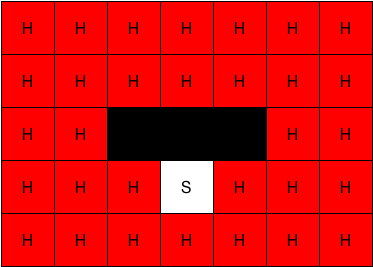
\includegraphics[width=.5\columnwidth]{./grid2.png}
  \caption{}
  \label{grid2}
\end{figure}
}

}



